


\thispagestyle{empty}


%~
%\tikz[remember picture, overlay] \node  at (current page.center){\includegraphics[width=\paperwidth,height=\paperheight]{images/titlebg}};


~
\vskip 1.75in

\begin{center}

\resizebox{.6\linewidth}{!}{\scshape Discrete}

\vskip -1ex

\resizebox{.9\linewidth}{!}{\scshape Mathematics}


\vskip 2em
\tikz[scale=0.55,yscale=.2]{\draw (0,0) rectangle (1,1);
\draw (1.4,0) rectangle (3.4, 1) (3.8,0) rectangle (4.8,1) (4.8,0) rectangle (5.8,1); \draw (6.2,0) rectangle (8.2,1) (8.2,0) rectangle (9.2,1) (9.6,0) rectangle (10.6,1) (10.6,0) rectangle (12.6,1) (13,0) rectangle (14,1) (14,0) rectangle (15,1) (15,0) rectangle (16,1);
}

\vskip 2em

\resizebox{.75\linewidth}{!}{\scshape An Open Introduction}


%\tikz[scale=0.55]{\draw (0,0) rectangle (1,1);
%\draw (1.4,0) rectangle (3.4, 1) (3.8,0) rectangle (4.8,1) (4.8,0) rectangle (5.8,1); \draw (6.2,0) rectangle (8.2,1) (8.2,0) rectangle (9.2,1) (9.6,0) rectangle (10.6,1) (10.6,0) rectangle (12.6,1) (13,0) rectangle (14,1) (14,0) rectangle (15,1) (15,0) rectangle (16,1);
%}

\vskip 1.5in

\resizebox{.35\linewidth}{!}{\scshape Oscar Levin}

\vskip .5in

\resizebox{.2\linewidth}{!}{\scshape 4th Edition}

\end{center}


%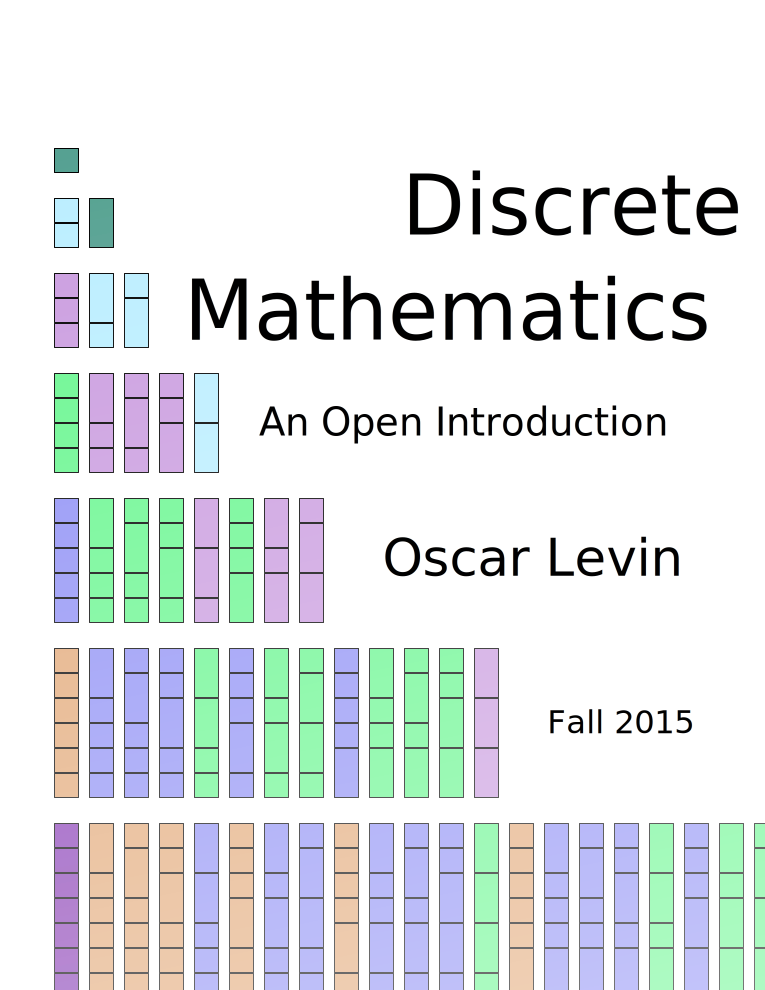
\includepdf[pages=-,pagecommand={\thispagestyle{empty}}]{frontmatter/cover2}
%
%

\clearpage






%\addtocontents{toc}{\protect\thispagestyle{plain}}
